\chapter{Related Work}
\label{ch:relatedwork}


In this chapter a simplification of the work done by \citet{chanetal} is presented followed by their original idea. The simplification is the primary work of this thesis. Conceptually, the original structure by \citet{chanetal} can be thought of as an extension of the simplified data structure. This way the reader will introduced to the concepts at an incremental level.\todo{rephrase} The theory behind a $kD$-tree will also be explained as it is the de facto standard of orthogonal range queries today and will be used to compare the practical results of the simplified model. \todo{rewrite}

The simplified model has a time complexity of $\mathcal{O}(\lg n)$ which is greather than the time complexity of the original model with $\mathcal{O}(\lg \lg n)$. However, the simplified model is far more simple - both in code and the data structures used. Because there is much more internal communication between the data structures in the original model and much more code to be executed, it is easy to assume \todo{Hvordan siger man det på engelsk?} that the running time constant of the original model far exceeds that of the simplified model, making the simplified faster than the original. \todo{rephrase}

Some sections will start with a \emph{preliminaries} subsection. This subsection will describe some of the auxiliary data structures used in the section.  This will make the reader acquinted with the data structures when they are referenced instead of having them explained in the middle of another explanation.

The algorithms mentioned in this chapter are all \emph{output-sensitive}, meaning that their running time depends on the amount of results found.

\section{kd-trees}

The current standard of range reporting is kd-trees. This technique will be used as a reference point when evaluting the results of the primary work in this thesis. With linear space it is an ideal data structure\todo{bedst kendt at virke i praksis} for range reporting on the RAM.

A kd-tree is constructed recursively: Given $n$ points, the median of the points with respect to x are found. All points which has an x-coordinate larger than the median goes to the right child, while points which has an x-coordinate smaller than the median, and the median point, goes to the left child. At the next level the points will be divided in a similar fashion, this time using the y-median and the y-coordinates instead. When dividing $n$ points, the median will be chosen as the $\lceil n/2 \rceil$-th smallest number \cite{compgeo}.
Switching back and forth between focussing on x or y is done at each level of the tree and this will be continued until a binary tree has been constructed with $n$ leaves.

The tree with $n$ points can be represented as flat array with $n$ entries. The $\lceil n/2 \rceil$-th element in the array is the root of the tree.
 With this in mind, the entire tree can represented using a flat array with $n$ elements. 
 \todo{Far from done - section needs work and rework}



\section{Simplified Range Searching}

\todo{Nu hvor jeg lige har beskrevet den originale, hvor meget skal jeg så gå i detaljer med hvorfor vi gør tingene? Som f.eks. at have tingene i rank space}

\subsection{Preliminaries}

\subsubsection{Predecessor search using binary search}
In order to find the rank space successor or rank space predecessor of a point, a binary search is used on a sorted array of points. This data structure uses $\mathcal{O}(n)$ space and have a query time of $\mathcal{O}(\lg n)$. By finding the first key that is bigger in the array, the index of that key is the rank space successor. By finding the last key that is smaller in the array, the index of that key is the ranks space predecessor.

\subsubsection{Succint rank queries}
Consider an array $A[1..n]$ with elements from some alphabet $\Sigma$. Given an index $i$ in the array, we want to find out how many elements in $A[1..i]$ is equal to $A[i]$. We call this a \emph{rank query}. We want to be able to answer the rank query in constant time. In order to do this checkpoints are created. For each character in the alphabet $\Sigma$, the checkpoint contains the number of times that character appears in $A[1..i]$, where $i$ is the checkpoint location. Such a checkpoint takes up $\mathcal{O}(\Sigma \lg n)$ space. By placing each checkpoint $\Sigma \lg n$ entries apart of each other, all of the checkpoints use $\mathcal{O}(\frac{n}{\Sigma \lg n} \cdot \Sigma \lg n) = \mathcal{O}(n)$ space.

Furthermore, for each entry in the array $A$, a smaller sum will be stored. Each entry in $A$ contains a character from the alphabet $\Sigma$. At $A[i]$ we store the amount of times the character at $A[i]$ appears since the last checkpoint. This is a smaller number and can be stored using $\mathcal{O}(\lg (\Sigma \lg n))$ bits per entry in $A$. This is because we only need $\lg x$ bits to store a number which has a maximum value of $x-1$. Since there is only $\Sigma \lg n$ entries between each checkpoint, this adds up. \todo{hvorfor passer det kun space bound hvis $\Sigma < \sqrt{\lg n}$?}

For smaller alphabets, we use another scheme. Checkpoinst are still stored at every $\Sigma \lg n$ positions. In addition to this, minor checkpoints are added. These minor checkpoints are added at every $\lg \lg n$ positions and contain amount of time each character is seen since the last major checkpoint. These minor checkpoints take up $\mathcal{O}(\Sigma \lg \lg n)$ each. In order to answer the rank query, a query to the last major checkpoint and the last minor checkpoint has to be made. 

\todo{hvorfor $\sqrt{\lg n}$ og $\sqrt{\lg n} \cdot \lg^2 \lg n$?}


\subsection{Solving the ball-inheritance problem} 
\label{ssection:solving-ball}

Consider a perfect binary tree with $n$ leaves. At each level a bit vector $A[1..n]$ is used to indicate which of a node's children a ball is inherited by: If $A[i]$ is $0$ means that the ball with identity $i$ in that node was inherited by its left child and $1$ means that it was inherited by its right child. Given a node and an identity of a ball we can know calculate the ball's identity in the node it is inherited by. The node can answer the query $rank(k) = \Sigma_{i \leq k} A[i]$. If a ball is inherited by the right child node its new identity at that node is $rank(i)$ because that is how many $1$'s that preceed it in the current node. If a ball is inherited by the left child node the new identity is then $i-rank(i)$. With this information it is possible to traverse down the tree following a ball from any given node to a leaf. There are $n$ balls per level which is represented by a bit vector of size $n$ bits per level. Even though conceptually this bit vector is divided out amongst the nodes of that level, we can interchangebly think of it as a bit vector per level or a bit vector per node.\todo{Rephrase and replace} Each level in the tree uses $\mathcal{O}(n)$ bits to store the bit vectors. This adds up to $\mathcal{O}(n \lg n)$ bits, or $\mathcal{O}(n)$ words in all. This trivial solution to the ball-inheritance problem uses $\mathcal{O}(\lg n)$ query time, given that it follows a ball $\mathcal{O}(\lg n)$ steps down to its leaf. The rank function is a constant time query.\todo{henvis til prelim}. \\


A bit vector is an array with entries from the alphabet $\Sigma = \{0,1\}$, where each entry is used to indicate whether a left or right child has been chosen to inherit a given ball. By expanding the alphabet we can point to the childrens children, $\Sigma = \{0,1,2,3\}$, the childrens childrens children, $\Sigma = \{0,1,2,3,4,5,6,7\}$, and so forth. Expanding the alphabet will use $\mathcal{O}(n \lg \Sigma)$ bits per level. Storing a pointer from level $i$ to level $i+\Delta$ increases the storage space by $\Delta$ bits per ball, but also enables the ball to be inherited by $2^\Delta$ descendants. By expanding the alphabet the query time can be lowered since it is possible to take bigger steps down the tree. 

Using this concept, we pick $B$ such that $2 \leq B \leq m$, where $m$ is the height of the tree. All levels that are a multiple of $B^i$ expand their alphabet such that the balls reach $B^i$ levels down. If a target level does not exist, the ball points to its leaf. We need at most visit $B$ levels that are multiple of $B^i$ before reaching a level that is multiple of $B^{i+1}$, making it possible to jump down the tree with bigger and bigger steps.

Storing the expanded alphabets at each level that is multiple of $B^i$ costs $B^i$ bits per ball. The total cost is then $\Sigma^{\lg_B \lg n}_i \frac{\lg n}{B^i} \cdot \mathcal{O}(B^i) = \mathcal{O}(\lg n \cdot \lg_B \lg n)$ bits per ball, at all levels. With $n$ balls, this is $\mathcal{O}(n \lg_B \lg n)$ words of space with query time of $\mathcal{O}(B \lg_B \lg n)$. \todo{Det er fordi $\lg_B \lg n$ er det største $i$ som beskriver $B^i \leq \lg n$ }



\subsection{Solving range reporting}

Consider a perfect binary tree with $n$ leaves. The root contains $n$ points in $2$-d rank space. These $n$ balls are sorted by their y-rank. When distributing the balls for inheritance, a node will give both its children half of its balls: the lower half sorted by the x-rank to its left child and the upper half by x-rank to its right child. The order of the balls in a child node will be the same as the parent node. \todo{rephrase} The actual coordinates of the balls are only stored at the leaves and we know that x-coordinates of the balls in the leaves are sorted from left to right - smallest to highest. Since the actual coordinate points are only stored once, this data structure uses linear space. \\

Given a range query $q = [x_1, x_2] \times [y_1, y_2]$ the rank successors of $x_1$ and $y_1$ and the rank predecessors of $x_2$ and $y_2$ are looked up. We know from section \todo{ref} that a range query can be translated to a rank space query. We call these $x^*_1, y^*_1, x^*_2$ and $y^*_2$. We use $x^*_1$ and $x^*_2$ to find the lowest common ancestor, $LCA(x^*_1, x^*_2)$, containing all the points between $x_1$ and $x_2$. \\

In the root we mark the position of $y^*_1$ and $y^*_2$ on the bit vector used to indicate which descendant a balls goes to. This range indicates which balls lie within the range of $[y_1, y_2]$. Going forward we will use $i$ and $j$ to indicate this range in the bit vector of any given node. When  a node inherits this range from a parent, the rank function is used to query how many points before $i$ went to this node, and how many points before $j$ went to this node. We refer to section \ref{ssection:solving-ball} \todo{refer to corret place} on how to update the positions using the rank query. This works because the points in a node are sorted by their y-rank and we keep track of how many points in a given node falls within the range of $[y_1, y_2]$ updating the range of $[i,j]$ everytime a node inherits balls. \todo{Skriv afsnit om} \\

We know the positions of the leaves containing $x^*_1$ and $x^*_2$ so we can traverse from the $LCA$ down to each of them. Traversing to $x^*_1$, the first stop is the left child of the $LCA$. From here, each time a node selects its left child as the path to $x^*_1$ we know that the subtree contained in the right child contains points between $x_1$ and $x_2$. Symmetrically, the same applies when going right from the $LCA$: Each time a node selects a right child on the path to $x^*_2$ the subtree contained in the left child contains points between $x_1$ and $x_2$. This concept is seen on figure \ref{fig:LCA}. \\

While keeping the y-rank range updated, we travel from the root to the $LCA$. From here we travel down to both $x^*_1$ and $x^*_2$. Each time a subtree between $x^*_1$ and $x^*_2$ is visited, know that it it fully included on the x-dimension. We can then look in its bit vector range to determine which of the balls refered to from this node is included in the y-dimension. For all the balls included in the y-dimension, we use the ball-inheritance structure to look up their actual coordinates in $\mathcal{O}(\lg^\epsilon n)$ time.

\begin{figure}[H]
    \centering
    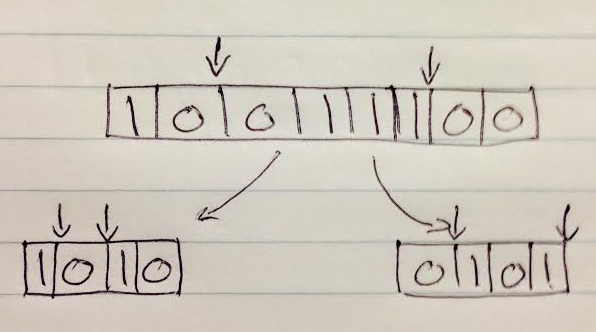
\includegraphics[width=0.6\textwidth]{pictures/bit_vector_split.png}
    \caption{When nodes inherit their bit vector ranges from their parent, it can become obvious if the entire subtree is contained within the range of $[y_1, y_2]$ or falls without the range.}
    \label{fig:bitvectorsplit}
\end{figure}


The data structure is utilized as follows:
\begin{enumerate}
    \item Use a binary seach to find the rank space predecessors and successors of $x_1$, $y_1$, $x_2$ and $y_2$. At this point the algorithm will terminate if either rank space range is empty.
    \item From $LCA(x^*_1, x^*_2)$, both $x^*_1$ and $x^*_2$ will be visited. The range y-rank range found in step $1$ will be updated from the root to this $LCA$ and updated from the $LCA$ to $x^*_1$, $x^*_2$ and all the subtrees between them.
    \item Each time a fully included subtree is visited, we determine which balls falls within the y-range and use the ball-inheritance structure to travel to its leaf. When a leaf is visited, its actual coordinates will be reported back as a result.
\end{enumerate}

The actual coordinates of the points are only stored at the leaves which then takes up $\mathcal{O}(n)$  words of space. The rest of the tree contains $\lg n$ levels of bit vectors of $n$ bits taking $\mathcal{O}(n \lg n)$ bits, $\mathcal{O}(n)$ words. Looking up the rank-space predecessor and successor of $x_1, x_2, y_1$ and $y_2$ using a simple binary search at the root requires $\mathcal{O}(n)$ space and $\mathcal{O}(\lg n)$ time. Summing it up, the entire data structure uses $\mathcal{O}(n)$ words of space. 

Walking from the root to the $LCA$ requires $\mathcal{O}(\lg n)$ steps. Visiting $x^*_1$ and $x^*_2$ requires $\mathcal{O}(\lg n)$ steps each. Visiting each of the $k$ leaves in the subtrees between $x^*_1$ and $x^*_2$ containing the points which will be reported as a result takes $\mathcal{O}(k \cdot \lg^\epsilon n)$ time. \todo{shorten sentence}

This adds up to $\mathcal{O}(\lg n + k\cdot\lg^\epsilon n)$ query time to report $k$ points as results. An empty range will be detected by the binary search at the root. If the binary search does not report an empty range, we proceed to use the algorithm. \\

\begin{figure}[H]
    \centering
    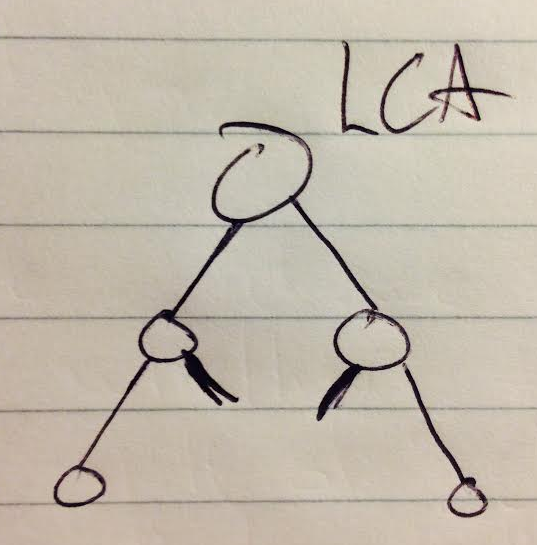
\includegraphics[width=0.6\textwidth]{pictures/LCA.png}
    \caption{Traversing left from the LCA, each right subtree contains x-coordinates between $x_1$ and $x_2$. Traversing right from the LCA the same holds for left subtrees.}
    \label{fig:LCA}
\end{figure}


\section{Orthogonal Range Searching}
\label{sect:original}
Utilizing the ball-inheritance structure, \citeauthor{chanetal} propose a better solution for orthogonal range search queries. With the same space complexity as the $kD$-tree, but lower query time. Theorem $2.1$ states that \emph{for any $2 \leq B \leq \lg^\epsilon n$, we can can solve $2$-d orthogonal range reporting in rank space with $\mathcal{O}(n \lg_B \lg n)$ space and $(1+k)\mathcal{O}(B \lg \lg n)$ query time.}

In this section some supporting data structures will be introduced. Then we will show how the ball-inheritance is used in conjunction with these data structures to find the points within a search query $q = [x_1, x_2] \times [y_1, y_2]$.

\subsection{Preliminaries}

\subsubsection{Range minimum queries}
In order to find the smallest element in a range, a succint data structure will be used. This data structure is said to solve the \emph{range minimum query} problem and will be refered to as RMQ. 
Consider an array $A$ with $n$ comparable keys, this data structure allows finding the index of the minimum key in the subarray $A[i,j]$. \todo{Describe either the cartesian tree or reference 29}. 
This range minimum data structure has a contant query time. \todo{Skal jeg indkludere samme reference som i \citet{chanetal} $[29]$?}

\subsubsection{Rank space predessecor search}
In order to look up the rank space predecessor of a given coordinate, another succint data structure will be used. This data structure has a smaller space complexity than the RMQ, but has a bigger query time.
Given a sorted array $A[1..n]$ of $\omega$-bit integers, predecessor search queries in $\mathcal{O}(\lg \omega)$ time is supported using $\mathcal{O}(n \lg \omega)$ space which has oracle access to the entries in the array. \todo{reference}. The points in rank space of $\mathcal{O}(\lg n)$ bits will use $\mathcal{O}(n \lg \lg n)$ bits per level, with $\omega = \lg n$, and $\mathcal{O}(n \lg n \lg \lg n)$ bits in all, which is $\mathcal{O}(n \lg \lg n)$ words. 

\subsection{Solving range reporting}
With a solution to the ball-inheritance problem, \citet{chanetal} proposes \textbf{Lemma 2.4} \emph{if the ball inheritance problem can be solved with space $S$ and query time $\tau$, $2$-d range reporting can be solved with space $\mathcal{O}(S+n)$ and query time $\mathcal{O}(\lg \lg n + (1+k) \tau)$.} \\


The ball distribution scheme of this data structure is the same as the simplified range search of section \ref{ssection:solving-ball}. Having distributed the $n$ points from the root to the leaves, additional data structures are required in order to answer the range queries. For each node in the tree that is a right child a range minimum query structure is added. The indices are the y-rank and the keys are the x-rank that the given node contains. A range maximum query structure is added to the all the nodes which are left children. Each data structure uses $2n + \mathcal{O}(n)$ bits, making it $\mathcal{O}(n)$ bits per level of the tree and $\mathcal{O}(n \lg n)$ bits in all - i.e. $\mathcal{O}(n)$ words of space. \\

There is still the matter of adding predecessor (and successor) search for the y-rank.
For this purpose the data structure described in subsection \todo{ref} is added to some levels of the tree. The rank space predessecor structure works on an array of the y-ranks, which is already sorted. In order to reduce this to linear space we will only place this predecessor search structure at levels which are multiples of $\lg \lg n$. When using the predecessor search from the lowest common ancestor of $x^*_1$ and $x^*_2$, $LCA(x^*_1, x^*_2)$, we go up to the closest ancestor to use its search structure. Searching takes $\mathcal{O}(\lg \lg n)$ time plus $\mathcal{O}(1)$ queries to the ball-inheritance structure: using the ball-inheritance structure we walk at most $\lg \lg n$ steps down while translating the ranks of $y_1$ and $y_2$ to the right and left child of $LCA(x^*_1, x^*_2)$. 

The reason why this structure is necessary for the y-ranks and not the x-ranks, is because of the way the points have been distributed in the ball-inheritance tree: From left to right, the leaves have x-rank $1,2,..n$ so we can easily locate a given range in x-dimension, but in order to keep track of the y-dimensional range we need to follow the balls down the ball-inheritance structure. Adding this structure to each $\lg \lg n$ level saves us from going all the way from the root down to the $LCA$. \todo{rephrase} \\

In order to use this new original data structure by \citet{chanetal} to report points in the range of $[x_1, x_2] \times [y_1, y_2]$ we follow these steps:
\begin{enumerate}
  \item We find the rank space successor of $x_1$, $x^*_1$, and the rank space predecessor of $x_2$, $x^*_2$. We use these to find the lowest common ancestor of $x^*_1$ and $x^*_2$, $LCA(x^*_1, x^*_2)$. This is the lowest node in the tree containing at least all the points between $x_1$ and $x_2$. By knowing $x^*_1$ and $x^*_2$, finding the lowest common ancestor is a constant time operation. Given that points are in an array, we can use xor as our $LCA$ operation. \todo{rephrase}
  \item As in step $1$ where we found the rank space of the x-coordinates, we find the rank space coordinates of the y-coordinates, $y^*_1$ and $y^*_2$, inside the left and right child of $LCA(x^*_1, x^*_2)$. This step is precisely what the rank space predecessor structure mentioned above supports.
  \item We now descend into the right child of $LCA(x^*_1, x^*_2)$ and use the range minimum query structure to the find the index $m$ (the y-rank) of the point with the smallest x-rank in the range $[y^*_1, y^*_2]$. Solving the ball-inheritance problem, we follow the path to the leaf to find the actual x-coordinate of the point. If the x-coordinate is smaller than $x_2$ we return the point as a result and recurse into the ranges of $[y^*_1, m-1]$ and $[m+1, y^*_2]$ in order to find more points. When this is done we apply the same concept to the left child of $LCA(x^*_1, x^*_2)$ using the range maximum query to find points above $x_1$.
\end{enumerate}

\todo{Insert figure to conceptually show we are working our way out from the inside}

The time complexity of step $3$ depends on the use of the ball-inheritance structure. The time to traverse this structure is dependent on the improvements made in \ref{ssection:solving-ball}. An empty range will result in two queries, one query to each child of $LCA(x^*_1, x^*_2)$. In the worst case the amount of queries to the ball-inheritance structure will not exceed twice the number of results reported. Each time a result is found, a recursion is made to both the left and right subrange of that result. If one of the sides constantly fails to find a result, two queries are made for each result found. 

Conceptually, $LCA(x^*_1, x^*_2)$ describes a point between $x_1$ and $x_2$. Step $3$ selects points that are in the range of $[y_1, y_2]$ moving outwards from the point of $LCA(x^*_1, x^*_2)$, always picking the point closest to $LCA(x^*_1, x^*_2)$ in its decreasing y-range. \todo{rephrase}

Going back to Lemma $2.4$, we see that the time complexity fits: $\mathcal{O}(\lg \lg n)$ time is used for the predecessor search and $\mathcal{O}((1+k)\tau)$ time is used for walking from the $LCA$ to the leaves solving the ball inheritance problem for the $k$ results.

The three approaches described above all use a number of bits linear to the amount of points. The original search structure by \citet{chanetal} is the fastest with its $(1+k)\mathcal{O}(B\lg \lg n)$ query while kd-trees are the slowest with $\mathcal{O}(\sqrt{n} + k)$ query time.

\todo{ADD CONSTANT TIME DIFFERENCE TALK}


